\documentclass[a4paper,oneside]{article}

\usepackage[utf8]{inputenc}
\usepackage[T2A]{fontenc}
\usepackage[english,russian]{babel}

\usepackage{amsmath}
\usepackage{mathtools}
\usepackage{amsfonts}
\usepackage{enumitem}
\usepackage{amsthm}
\usepackage{minted}
\setminted{fontsize=\small, breaklines=true, style=emacs, linenos}
\usepackage{graphicx}
\graphicspath{ {./images/} }
\usepackage{float}

\newtheorem{theorem}{Теорема}[subsection]
\newtheorem*{theorem*}{Теорема}

% --- Определение --- %
\theoremstyle{definition}
\newtheorem{definition}{Определение}[subsection]
\newtheorem*{definition*}{Определение}
% ------------------- %

\title{{Теория кодирования и сжатия информации}\\{Лабораторная работа №3}}
\author{Гущин Андрей, 431 группа, 1 подгруппа}
\date{\the\year{} г.}

\begin{document}

\maketitle

\section{Задача}

Разработать программу осуществляющую архивацию и разархивацию текстового файла
используя алгоритм Шеннона. Программы архивации и разархивации должны быть
представлены отдельно и работать независимо друг от друга. Определить для
данного шифра характеристики 1 (коэффициент сжатия) и 2 (скорость сжатия). К
работе необходимо прикрепить отчет и программный проект.


\section{Алгоритм}

Алгоритм Шеннона заключается в создании нового кода для каждого встречающегося
в тексте символа на основе частоты встречи этого символа.

Алгоритм состоит из следующих шагов:
\begin{enumerate}
  \item Вычислить частоты $p_i$ всех встретившихся символов;
  \item Отсортировать полученный список по невозрастанию;
  \item Вычислить префиксные суммы $b_i$ для списка частот;
  \item Перевести префиксные суммы из десятичной системы счисления в двоичную;
  \item
    В качестве кода для символа $i$ необходимо использовать первые
    $\lceil -\log_2 p_i \rceil$ двоичных цифр после запятой из $b_i$.
\end{enumerate}


\section{Тестирование}

Для проверки программы были использованы тестовые тексты 1 (рис.
\ref{fig:test_1}) и 6 (рис. \ref{fig:test_6}). Можно заметить,
что после распаковки архива полученный файл совпадает с исходным (проверка
с помощью утилиты diff). Также можно заметить, что для файлов малого размера
архив увеличивает их размер за счёт метаданных.

\begin{figure}[H]
  \centering
  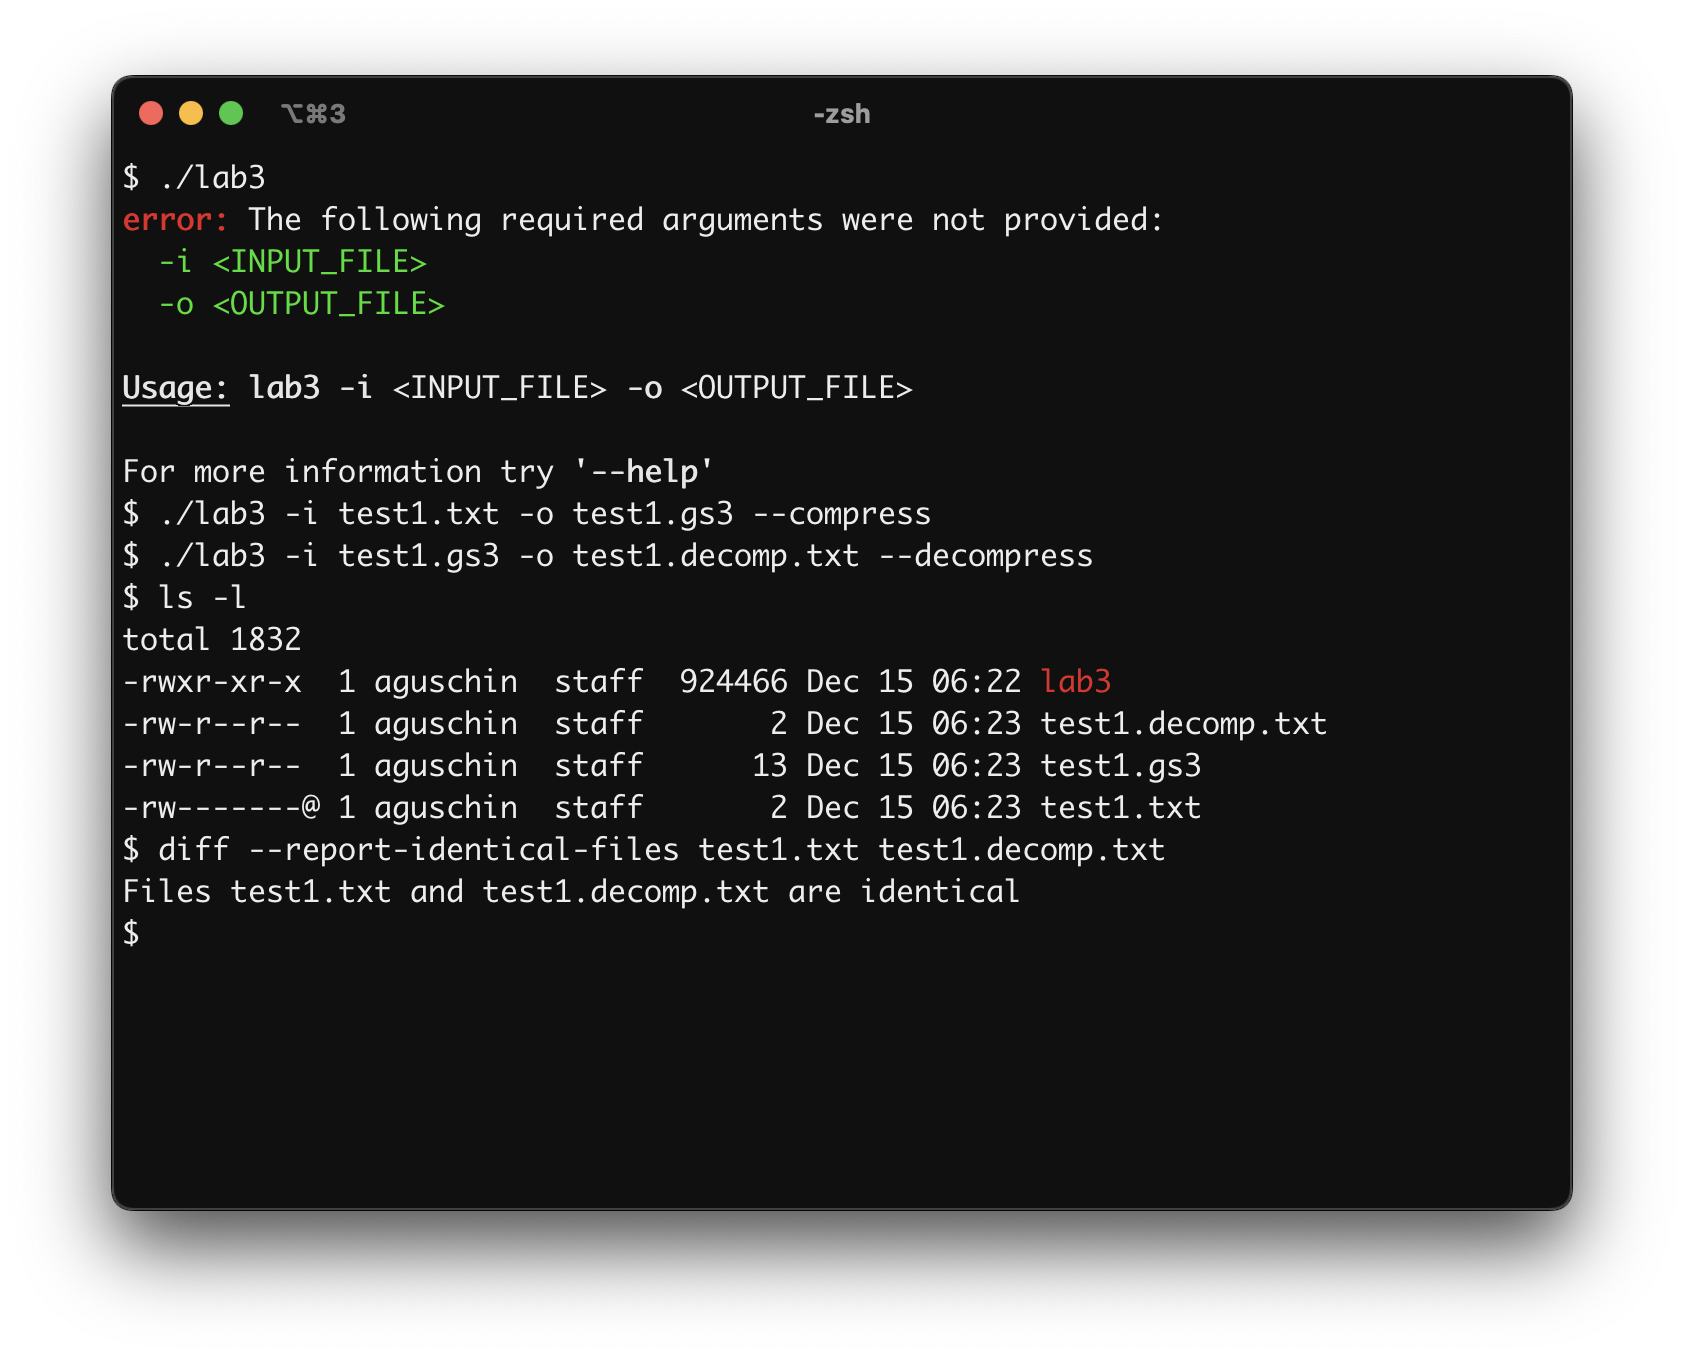
\includegraphics[width=0.9\textwidth]{test1.png}
  \caption{Сжатие текста Тест\_1.txt}
  \label{fig:test_1}
\end{figure}

\begin{figure}[H]
  \centering
  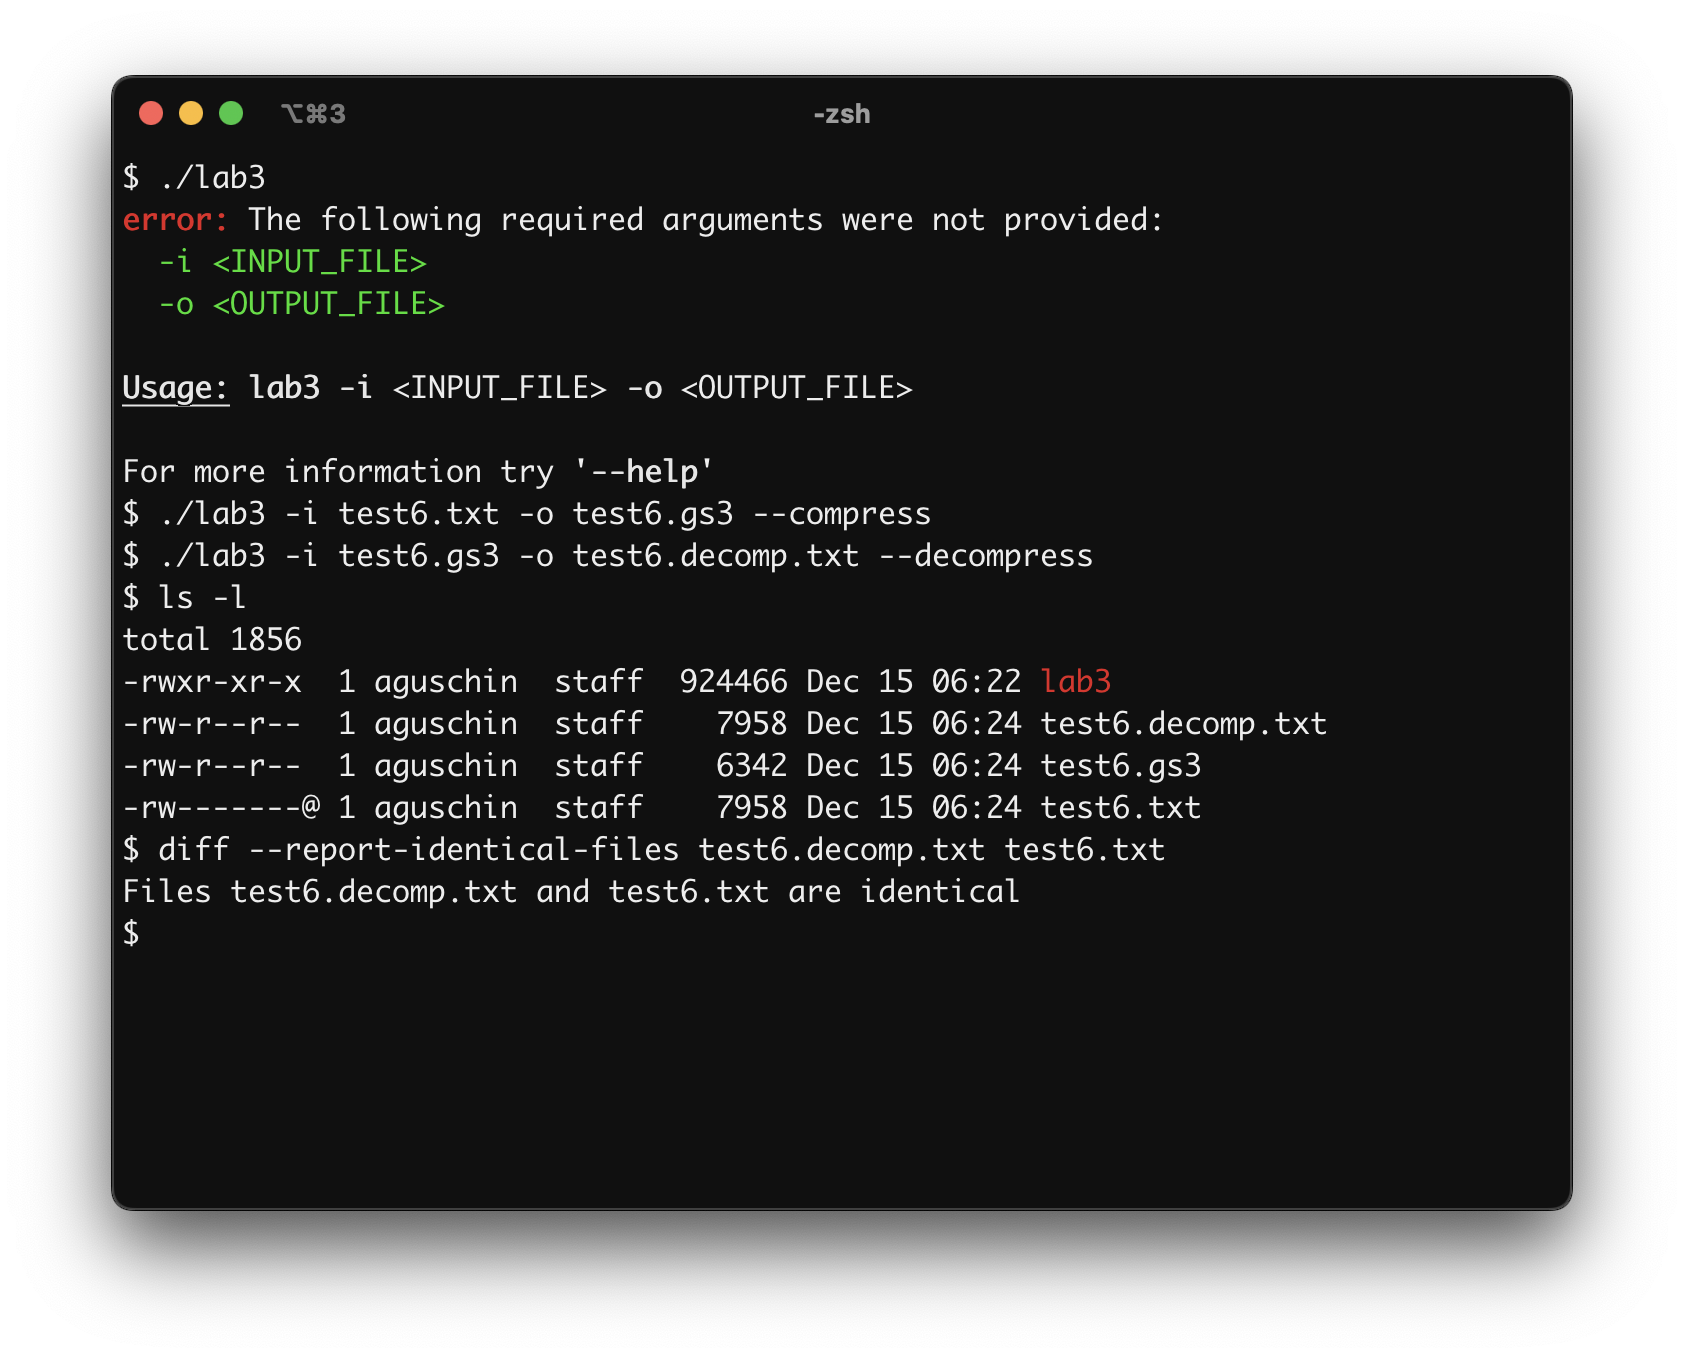
\includegraphics[width=0.9\textwidth]{test6.png}
  \caption{Сжатие текста Тест\_6.txt}
  \label{fig:test_6}
\end{figure}


\section{Вычисленные характеристики}

\subsection{Характеристика 1 (Коэффициент сжатия)}

Результаты применения программы к каждому из тестовых текстовых файлов занесены
в таблицу \ref{tbl:results}. Можно заметить, что в некоторых случаях архивация с
помощью алгоритма Хаффмана является неэффективной.

\begin{table}[H]
  \small
  \centering
  \begin{tabular}{|c|c|c|c|}
    \hline
    Название     & Исходный размер, байт & Сжатый размер, байт & Коэффициент \\ \hline \hline
    Тест\_1.txt  & 2           & 13          & 0.15385   \\ \hline
    Тест\_2.txt  & 33          & 192         & 0.17188   \\ \hline
    Тест\_3.txt  & 2739        & 2222        & 1.23267   \\ \hline
    Тест\_4.txt  & 330         & 54          & 6.11111   \\ \hline
    Тест\_5.txt  & 59          & 342         & 0.17251   \\ \hline
    Тест\_6.txt  & 7958        & 6342        & 1.25481   \\ \hline
    Тест\_7.txt  & 138245      & 91392       & 1.51266   \\ \hline
    Тест\_8.txt  & 574426      & 363679      & 1.57949   \\ \hline
    Тест\_9.txt  & 2752        & 352         & 7.81818   \\ \hline
    Тест\_10.txt & 2814        & 416         & 6.76442   \\ \hline
  \end{tabular}
  \caption{результаты тестирования}
  \label{tbl:results}
\end{table}

\subsection{Характеристика 2 (Скорость сжатия)}

Для тестирования скорости сжатия использовался произвольный двоичный
файл размера 76450438 байт ($\approx$73 мегабайта). В результате пяти
последовательных запусков, среднее время запаковки файла составило 3.45
секунд, среднее время распаковки составило 180 секунд.

Таким образом, средняя скорость сжатия составила 21.13299 Мбайт в секунду, а
средняя скорость разжатия составила 0.40505 Мбайт в секунду.


\section{Реализация}

Программа реализована на языке программирования Rust с использованием библиотеки
clap для чтения параметров командной строки. Сборка производится с помощью
программы cargo, поставляющейся вместе с языком.

\subsection{Содержимое файла shannon.rs}
\inputminted{rust}{../../lab3/src/shannon.rs}

\subsection{Содержимое файла main.rs}
\inputminted{rust}{../../lab3/src/main.rs}

\subsection{Содержимое файла Cargo.toml}
\inputminted{toml}{../../lab3/Cargo.toml}

\end{document}
